In this section we present the most important use cases of the eMall. Every use case has also associated a sequence diagram, but we decided to present only the most relevant situations of the use case in the sequence diagrams, so they do not contain all the possible alternatives. We also provide some use cases diagrams in order to better show the relationship between the actors and the actions that they can perform in the system, displaying the features and the capabilities of the application.
The following use cases are also related to the scenarios explained in the last chapter, formalizing the situations previously described. 

\subsection{Unregistered and registered EVD's use cases}
\begin{figure}[H]
    \centering
    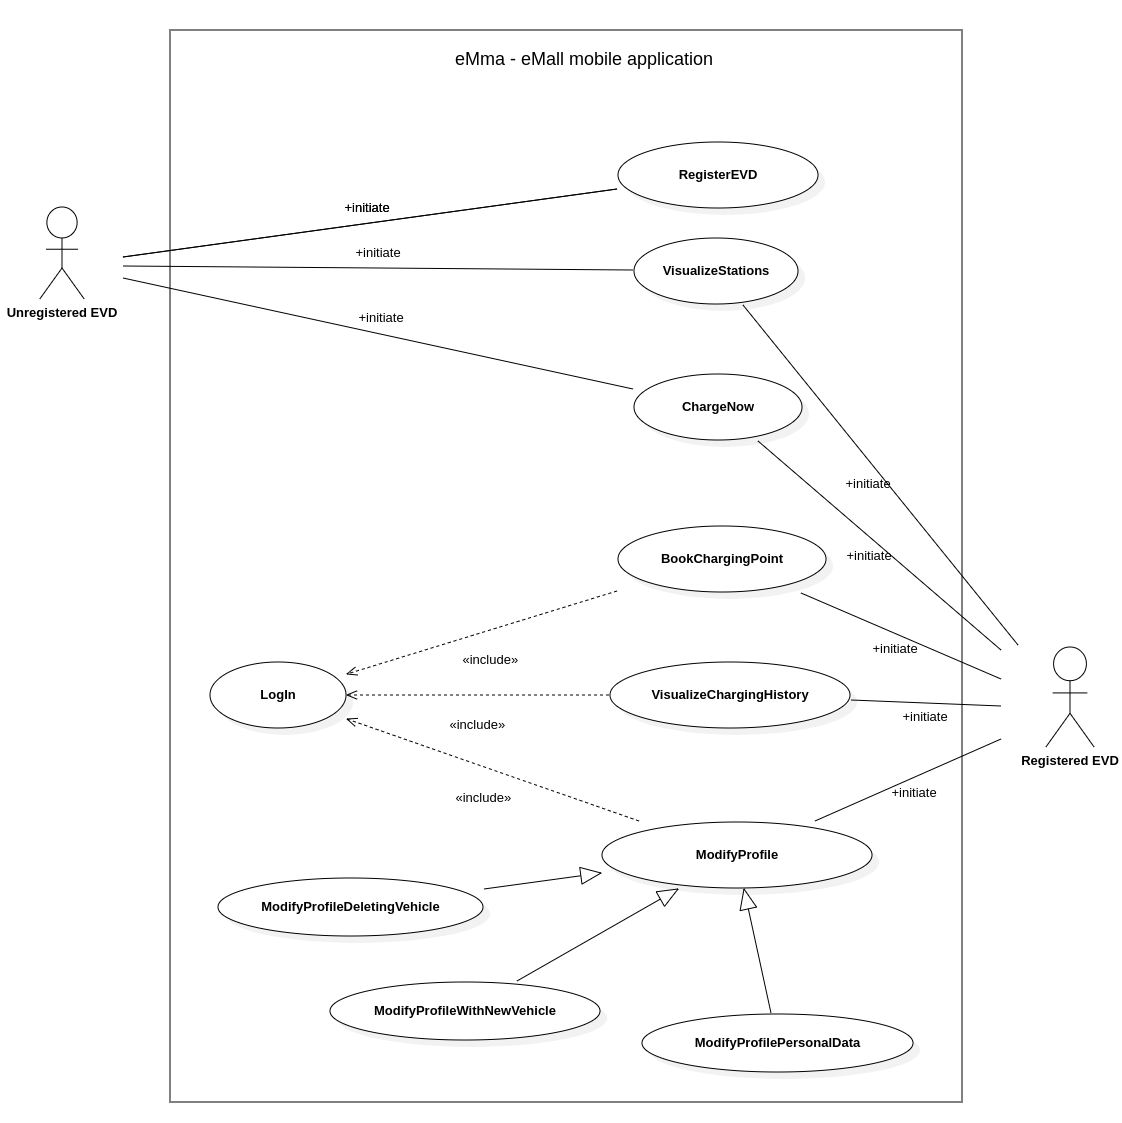
\includegraphics[width=1\textwidth]{Images/cp3/UseCaseDiagramEVD.png}
    \caption{Use cases diagram of the registered and unregistered EVD}
\end{figure}

%TODO: @Fabio complete the following 3 use cases
\paragraph{A new user registers into eMma}
\begin{center}
    \begin{longtable}{p{4cm} p{11cm}}
    \multicolumn{2}{r}{\itshape{Continue to the next page}}\\
    \endfoot
    \\
    \endlastfoot
    \hline
     Use case name &  RegisterEVD\\
     \hline
     Actor & Unregistered EVD \\
     \hline
     Entry condition & True \\
     \hline
     Event flow & 
         1. User opens the eMma mobile application \newline
         2. User starts the registering process \newline
         3. Users enters his personal data: name, surname, email \newline
         4. System check if the email is in the correct format \newline
         5. User creates a new password and confirms it a second time \newline
         6. System checks the security property of the password
         7. System verifies the property of the email \newline
         8. System ask the user for the consent to use his geographical location \newline
         9. User agrees \newline
         10. System ask the user to agree to terms of service \newline
         11. User agrees \newline
         12. the system starts <<include>> "ModifyProfileWithNewVehicle" at step 6 \newline
         13. the system ask for the user the payment details \newline
         14. The user insert the payment details \newline
         15. The system check the correctness of the inserted information \newline
         16. System creates new account and log in the user\\
     \hline
     Exit condition &  A valid account is created and the system logs in the user \\
     \hline
     Exceptions &  
        4a. The email confirmation process fails:
            \begin{adjustwidth}{1cm}{}
            1. The system shows an error on the email field and asks for a new email\newline
            2. User enters a new email
            \end{adjustwidth}
        6a. Password doesn't respect security requirements:
            \begin{adjustwidth}{1cm}{}
            1. The system ask the user for a new password \newline
            2. The user inserts a new password
            \end{adjustwidth}
        7a. User doesn't confirm the property of the email:
            \begin{adjustwidth}{1cm}{}
            1. The system deletes user's information after 10 minutes
            \end{adjustwidth}
        9/11a. User doesn't agree:
            \begin{adjustwidth}{1cm}{}
            1. The registration process doesn't proceed and after 10 minutes the system deletes user's information
            \end{adjustwidth}
        
     \\
     \hline
     Special requirements &  \\
     \hline
    \caption{RegisterEVD}
    \label{tab:RegisterEVD}
    \end{longtable}
\end{center}

\paragraph{Booking a charging point}
\begin{center}
    \begin{longtable}{p{4cm} p{11cm}}
    \multicolumn{2}{r}{\itshape{Continue to the next page}}\\
    \endfoot 
    \\
    \endlastfoot
    \hline
     Use case name &  BookChargingPoint\\
     \hline
     Actor & EVD \\
     \hline
     Entry condition &   The EVD is logged in the eMma and on the homepage\\
     \hline
     Event flow &
        1. EVD selects a charging station in the map \newline
        2. The system shows a view of all the available and free charging point sockets. For each socket information such as charging type (AC/DC), socket type, the charging speed, the price for kWh.
        3. 
        \\
     \hline
     Exit condition &  \\
     \hline
     Exceptions &  \\
     \hline
     Special requirements &  \\
     \hline
    \caption{BookingChargingPoint}
    \label{tab:BookingChargingPoint}
    \end{longtable}
\end{center}

\paragraph{Visualize charging history}
\begin{center}
    \begin{longtable}{p{4cm} p{11cm}}
    \multicolumn{2}{r}{\itshape{Continue to the next page}}\\
    \endfoot 
    \\
    \endlastfoot
    \hline
     Use case name &  VisualizeChargingHistory\\
     \hline
     Actor & Registered EVD \\
     \hline
     Entry condition &  \\
     \hline
     Event flow &  \\
     \hline
     Exit condition &  \\
     \hline
     Exceptions &  \\
     \hline
     Special requirements &  \\
     \hline
    \caption{VisualizeChargingHistory}
    \label{tab:VisualizeChargingHistory}
    \end{longtable}
\end{center}

\paragraph{Log in the system}
\begin{center}
    \begin{longtable}{p{4cm} p{11cm}}
    \multicolumn{2}{r}{\itshape{Continue to the next page}}\\
    \endfoot 
    \\
    \endlastfoot
    \hline
     Use case name &  LogIn\\
     \hline
     Actor & Registered user (EVD or CPO)\\
     \hline
     Entry condition &  The user is not logged in the system and wants to log in\\
     \hline
     Event flow &   1. The user accesses the eMall \newline
                    2. The eMall shows the log in page \newline
                    3. The user inserts the log in details \newline
                    4. The user clicks on the 'Sign In' button \\
     \hline
     Exit condition & The user is logged in and is shown the homepage of the eMall system \\
     \hline
     Exceptions &  If the credentials are not correct, after clicking the 'Sign In' button the user receives an error message and the log in is not successful \\
     \hline
     Special requirements &  After clicking the 'Sign In' button the eMall homepage must be shown in less than 2 seconds \\
     \hline
    \caption{LogIn}
    \label{tab:LogIn}
    \end{longtable}
\end{center}

\paragraph{Start a charging session}
\begin{center}
    \begin{longtable}{p{4cm} p{11cm}}
    \multicolumn{2}{r}{\itshape{Continue to the next page}}\\
    \endfoot 
    \\
    \endlastfoot
    \hline
     Use case name &  ChargeNow\\
     \hline
     Actor & EVD \\
     \hline
     Entry condition & The EVD is on the homepage of the eMma and the status of the charging point is free \\
     \hline
     Event flow &   1. The EVD clicks on the 'Charge now' button \newline
                    2. The EVD inserts the eMci code in the eMma and confirms the operation \newline
                    3. The eMall checks the correctness of the code and unlocks the charging point \newline
                    4. The system changes the status of the charging point from free to occupied \newline   
                    5. The EVD plugs in the connector \\
     \hline
     Exit condition &  The system starts the charging session \\
     \hline
     Exceptions &   1. If the EVD doesn't insert the correct code, the eMall doesn't unlock the chargin                         point and the eMma returns a warning message, allowing the user to reinsert the                         code\newline
                    2. If the user doesn't insert the plug in less than 5 minutes, the operation is deleted, and the charging point status return to free \\ 
     \hline
     Special requirements & After inserting the code, the eMall does all the necessary checks and changes the status of the charging point in less than 2 seconds, so the service can be perceived as fast and responsive. Also, the system has to start the charging of the EVD in less than 2 seconds, for the same reason \\
     \hline
    \caption{ChargeNow}
    \label{tab:ChargeNow}
    \end{longtable}
\end{center}

\paragraph{Update profile details adding a new vehicle}
\begin{center}
    \begin{longtable}{p{4cm} p{11cm}}
    \multicolumn{2}{r}{\itshape{Continue to the next page}}\\
    \endfoot 
    \\
    \endlastfoot
    \hline
     Use case name &  ModifyProfileWithNewVehicle\\
     \hline
     Actor & Registered EVD \\
     \hline
     Entry condition & The EVD is logged in the eMma and on the homepage \\
     \hline
     Event flow &   1. The EVD clicks on the 'Profile page' \newline
                    2. The system shows the profile page with personal information and EV's details \newline
                    3. The EVD clicks on the 'Update' button \newline
                    4. The eMma shows a page with different buttons from which to choose the update action \newline
                    5. The EVD clicks on the 'Add new vehicle' button \newline
                    6. The mobile app shows a form titled 'New EV' with different fields to fill up, in a semi-guided way \newline
                    7. The EVD inserts the data about the new EV: inserts the type of EV, the supported inlet type of the EV and the presence of the rectifier, the capacity of the battery, the supported power levels and the supported current levels \newline
                    8. The EVD clicks on the 'Ok' button to submit the form \newline
                    9. The eMall saves the data and associates them to the EVD's profile \newline
                    10. The system reloads the profile page with the new vehicle information \\
     \hline
     Exit condition &  The new EV is associated to the user information already saved in the system, and the eMma reloads the profile page with the new EV's details\\
     \hline
     Exceptions &   1. If the EVD doesn't insert all the mandatory information, after clicking the 'Ok' button the                     system gives an explicit error message with the missing data, and the user can continue to                       complete the form \newline
                    2. If at any time the user wants to exit the form, the application allows it, but all the data inserted so far are lost \\
     \hline
     Special requirements & After clicking the 'Ok' button the system has to save the data and reload the profile page in less than 10 seconds \\
     \hline
    \caption{ModifyProfileWithNewVehicle}
    \label{tab:ModifyProfileWithNewVehicle}
    \end{longtable}
\end{center}

\paragraph{Update profile details deleting vehicle}
\begin{center}
    \begin{longtable}{p{4cm} p{11cm}}
    \multicolumn{2}{r}{\itshape{Continue to the next page}}\\
    \endfoot 
    \\
    \endlastfoot
    \hline
     Use case name &  ModifyProfileDeletingVehicle\\
     \hline
     Actor & Registered EVD \\
     \hline
     Entry condition & The EVD is logged in the eMma and on the homepage \\
     \hline
     Event flow &   1. The EVD clicks on the 'Profile page' \newline
                    2. The system shows the profile page with personal information and EV's details \newline
                    3. The EVD clicks on the 'Update' button \newline
                    4. The eMma shows a page with different buttons from which to choose the update action \newline
                    5. The EVD clicks on the 'Delete vehicle' button \newline
                    6. The mobile app shows the list of the registered vehicles \newline
                    7. The EVD selects the EV he wants to delete \newline
                    8. The EVD clicks on the 'Ok' button to submit his choice \newline
                    9. The eMall retrieves the data of the user and deletes the selected vehicle \newline
                    10. The system reloads the profile page, in which the deleted vehicle is no more present \\
     \hline
     Exit condition &  The EV is deleted from the data associated to the EVD and the profile page is reloaded \\
     \hline
     Exceptions &   1. If the EVD doesn't select an EV to delete from the list, after clicking the 'Ok' button the                     system gives an error message, and the user has to select a vehicle or cancel the operation                     \newline
                    2. If the user wants to exit without selecting an EV, the application allows it, and no vehicle will be deleted from the profile\\
     \hline
     Special requirements & After clicking the 'Ok' button the system has to delete the vehicle from the EVD's data and reload the profile page in less than 3 seconds \\
     \hline
    \caption{ModifyProfileDeletingVehicle}
    \label{tab:ModifyProfileDeletingVehicle}
    \end{longtable}
\end{center}

\paragraph{Update profile modifying personal data}
\begin{center}
    \begin{longtable}{p{4cm} p{11cm}}
    \multicolumn{2}{r}{\itshape{Continue to the next page}}\\
    \endfoot 
    \\
    \endlastfoot
    \hline
     Use case name &  ModifyProfilePersonalData\\
     \hline
     Actor & Registered EVD \\
     \hline
     Entry condition & The EVD is logged in the eMma and on the homepage \\
     \hline
     Event flow &   1. The EVD clicks on the 'Profile page' \newline
                    2. The system shows the profile page with personal information and EV's details \newline
                    3. The EVD clicks on the 'Update' button \newline
                    4. The eMma shows a page with different buttons from which to choose the update action \newline
                    5. The EVD clicks on the 'Update profile' button \newline
                    6. The mobile app shows a form, already filled up with the personal data \newline
                    7. The EVD can modify the elements of the form, for example the email, the name, the payment details \newline
                    8. The EVD, after modifying some data, clicks on the 'Ok' button to submit the form \newline
                    9. The eMall checks the new data and through external APIs sends verification messages to the EVD \newline
                    10. The EVD confirms the verification messages from external applications, such as the email or the payment account \newline
                    11. The system, once received the confirmation, reloads the eMma page with a final confirmation page \newline
                    12. The EVD clicks the 'Confirm' button \newline
                    13. The eMall updates the data that have been changed, saving the correct information associated to the EVD's profile \newline
                    14. The system reloads the profile page with the new personal data \\
     \hline
     Exit condition & The system saves the new data, discarding the old ones, and the eMma reloads the profile page with the updated personal details\\
     \hline
     Exceptions &   1. If the EVD doesn't change any data of the form, after clicking the 'Ok' button the system                        reloads the profile page showing all the data present before the operation \newline
                    2. If at any time the user wants to exit the form, the application allows it, but all the data inserted so far are lost, keeping the last personal details \newline
                    3. If the EVD doesn't confirm the operation from the eMma or from the external applications, the updating request is deleted after 10 minutes, and the operation has to be restarted 
                    \\
     \hline
     Special requirements & After clicking the 'Confirm' button the system has to save the updated data and reload the profile page in less than 10 seconds \\
     \hline
    \caption{ModifyProfilePersonalData}
    \label{tab:ModifyProfilePersonalData}
    \end{longtable}
\end{center}

\paragraph{Visualize charging stations on the map}
\begin{center}
    \begin{longtable}{p{4cm} p{11cm}}
    \multicolumn{2}{r}{\itshape{Continue to the next page}}\\
    \endfoot 
    \\
    \endlastfoot
    \hline
     Use case name &  VisualizeStations\\
     \hline
     Actor & Registered EVD or unregistered EVD \\
     \hline
     Entry condition & The EVD is on the eMma homepage \\
     \hline
     Event flow &   1. On the homepage the eMma shows the map of the territory, based on the location shared by the mobile phone of the EVD \newline
                    2. The EVD clicks on the map \newline
                    3. The map shows the charging stations nearby the position on which the EVD clicked \newline
                    4. The EVD clicks on one of the charging stations presented on the map \newline
                    5. The eMma shows a page with the information related to the selected charging station: shows the name of the charging station with the relative rating reviews, the available chargers with their type of connectors, and the button 'Book now'\\
     \hline
     Exit condition & The EVD exits the homepage or closes the application \\
     \hline
     Exceptions &   1. If the EVD clicks on the map on an area without charging stations, no charging station will appear on the map \newline
                    2. If at any time the user wants to exit the eMma, the application allows it, and at the following access the action restarts from the homepage \\
     \hline
     Special requirements & After the EVD clicks on the map, the charging stations are shown in less than 2 seconds. As well, when the EVD clicks on the charging stations the related data are shown in less than 2 seconds, so the application can be perceived as fast and responsive \\
     \hline
    \caption{VisualizeStations}
    \label{tab:VisualizeStations}
    \end{longtable}
\end{center}

\subsection{CPO's use cases}
\begin{figure}[H]
    \centering
    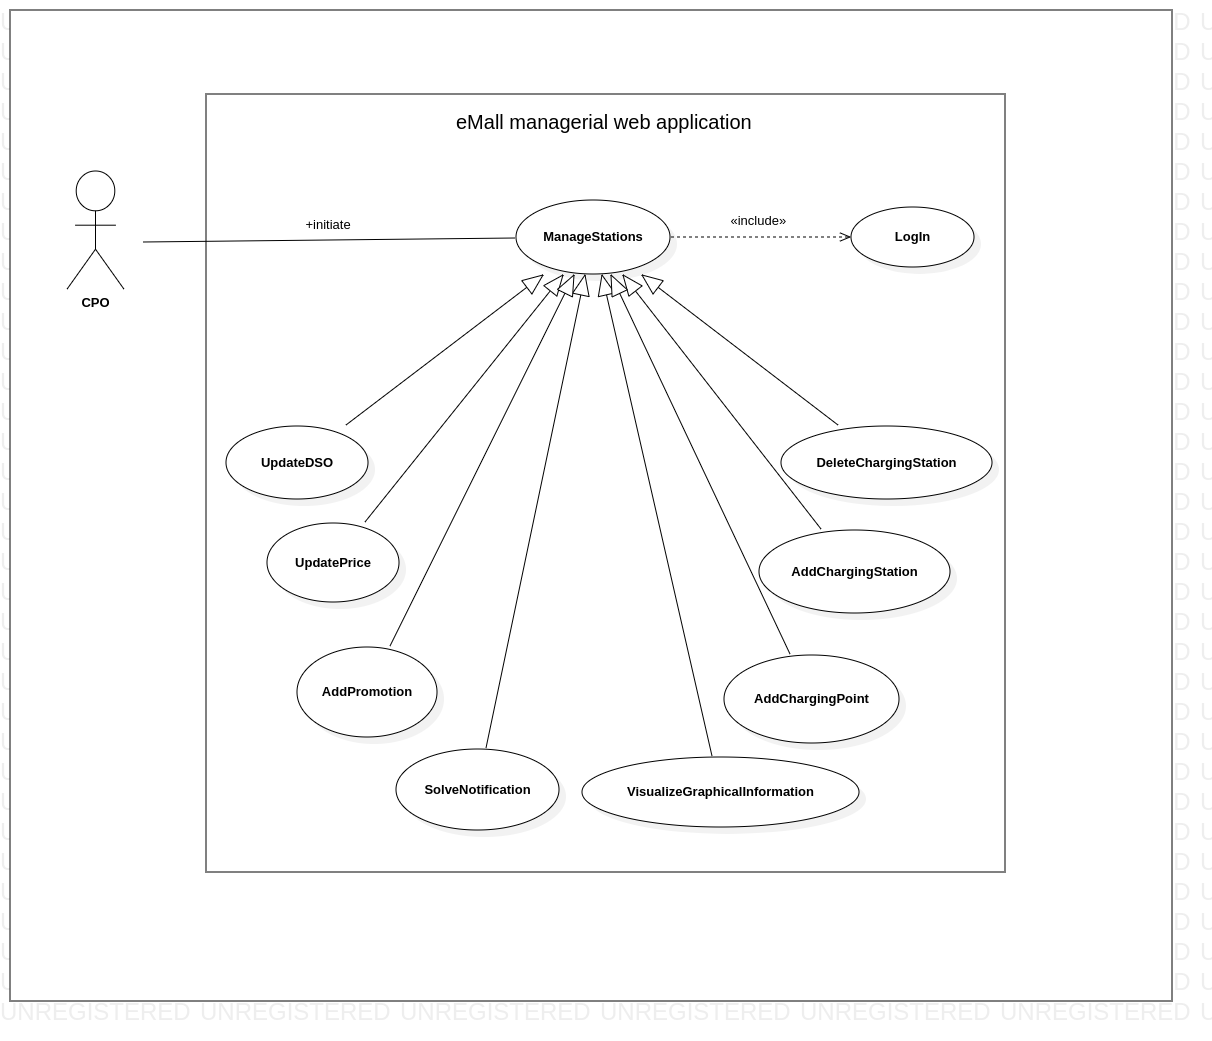
\includegraphics[width= 0.9\textwidth, trim={2cm 5cm 5cm 3cm}, clip]{Images/cp3/UseCaseDiagramCPO.png}
    \caption{Use cases diagram of the CPO}
\end{figure}
\paragraph{Manage the charging stations}
\begin{center}
    \begin{longtable}{p{4cm} p{11cm}}
    \multicolumn{2}{r}{\itshape{Continue to the next page}}\\
    \endfoot 
    \\
    \endlastfoot
    \hline
     Use case name &  ManageStations\\
     \hline
     Actor & CPO \\
     \hline
     Entry condition & The CPO is logged in the web application of the eMall and on the homepage \\
     \hline
     Event flow &   1. On the homepage the eMall shows to the CPO the charging stations associated to the company                   registration and any notification on the stations \newline
                    2. The CPO clicks on a charging station or on a notification \newline 
                    3. The system shows a form with the details of the charging station and if there are notifications regarding the station the interested parts of the form are highlighted in red \newline
                    4. The CPO can click on any part of the form and modify the data of the station \newline
                    5. The CPO clicks the 'Confirm' button \newline
                    6. The system checks and saves the new data related to the charging station \newline
                    7. The system sends a notification message informing of the success of the operation \newline
                    8. The system loads a page showing the charging station with the new associated information\\
     \hline
     Exit condition &  The CPO closes the page loaded by the system with the updated data of the charging station, returning to the homepage \\
     \hline
     Exceptions &   1. If the CPO doesn't modify anything on the form before submitting it, the eMall sends a                       message which informs that the data have not been modified, and returns to the homepage \newline
                    2. If at any time the CPO wants to exit, the application allows it, and no changes will be applied if the procedure wasn't completed \\
     \hline
     Special requirements & After the CPO clicks on the 'Confirm' button, the charging station with the related details is updated and shown on a new page in less than 2 seconds, in order for the application to be perceived as fast and responsive \\
     \hline
    \caption{ManageStations}
    \label{tab:ManageStations}
    \end{longtable}
\end{center}
The use case about the CPO managing the charging stations, is a generic use case, that can be further analyzed considering the actions that the CPO actually performs on the system, to manage the stations. In the following use cases, we specialize some of these interactions, showing available functionalities of the web application of the eMall. The sequence diagrams of the next use cases are similar to the one reported for the general interaction of the CPO with the system, so they will not be added to this document.

\paragraph{Update the DSO of a charging station}
\begin{center}
    \begin{longtable}{p{4cm} p{11cm}}
    \multicolumn{2}{r}{\itshape{Continue to the next page}}\\
    \endfoot 
    \\
    \endlastfoot
    \hline
     Use case name &  UpdateDSO\\
     \hline
     Actor & CPO \\
     \hline
     Entry condition & The CPO is logged in the web application of the eMall and on the homepage \\
     \hline
     Event flow &   1. On the homepage the eMall shows to the CPO the charging stations associated to the company                   registration and any notification on the stations \newline
                    2. The CPO clicks on a charging station \newline 
                    3. The system shows a form with the details of the charging station \newline
                    4. The CPO clicks on the 'DSO' cell present in the form \newline
                    5. The system shows a new sub-page with the available DSOs and the respective information: for each DSO the page shows the energy resources, their capacity and their prices \newline
                    6. The CPO selects the DSO and the energy source he wants to use for the charging station \newline
                    7. The CPO clicks on the 'Ok' button \newline
                    8. The web application returns to the form of the charging station with the new selected DSO information replacing the previous one \newline
                    9. The CPO clicks the 'Confirm' button \newline
                    10. The system checks and saves the new data related to the charging station \newline
                    11. The system sends a notification message informing of the success of the operation \newline
                    12. The system loads a page showing the charging station with the new associated information\\
     \hline
     Exit condition &  The CPO closes the page loaded by the system with the updated data of the charging station, returning to the homepage \\
     \hline
     Exceptions &   1. If the CPO doesn't modify anything on the form before submitting it, the eMall sends a                       message which informs that the data have not been modified, and returns to the homepage \newline
                    2. If at any time the CPO wants to exit, the application allows it, and no changes will be applied if the procedure wasn't completed \\
     \hline
     Special requirements & After the CPO clicks on the 'Confirm' button, the charging station with the related details is updated and shown on a new page in less than 2 seconds, in order for the application to be perceived as fast and responsive \\
     \hline
    \caption{UpdateDSO}
    \label{tab:UpdateDSO}
    \end{longtable}
\end{center}

\paragraph{Update the price of a charging station}
\begin{center}
    \begin{longtable}{p{4cm} p{11cm}}
    \multicolumn{2}{r}{\itshape{Continue to the next page}}\\
    \endfoot 
    \\
    \endlastfoot
    \hline
     Use case name &  UpdatePrice\\
     \hline
     Actor & CPO \\
     \hline
     Entry condition & The CPO is logged in the web application of the eMall and on the homepage \\
     \hline
     Event flow &   1. On the homepage the eMall shows to the CPO the charging stations associated to the company                   registration and any notification on the stations \newline
                    2. The CPO clicks on a charging station \newline 
                    3. The system shows a form with the details of the charging station \newline
                    4. The CPO changes the price of the charging station from the form \newline
                    5. The CPO clicks the 'Confirm' button \newline
                    6. The system checks and saves the new data related to the charging station \newline
                    7. The system sends a notification message informing of the success of the operation \newline
                    8. The system loads a page showing the charging station with the new associated information\\
     \hline
     Exit condition &  The CPO closes the page loaded by the system with the updated data of the charging station, returning to the homepage \\
     \hline
     Exceptions &   1. If the CPO doesn't modify anything on the form before submitting it, the eMall sends a                       message which informs that the data have not been modified, and returns to the homepage \newline
                    2. If the price doesn't respect a level fixed by the company policy, the system sends an error message, informing the CPO that the price is to high or too low, and the CPO has to modify again the form, otherwise no change will be applied \newline
                    3. If at any time the CPO wants to exit, the application allows it, and no changes will be applied if the procedure wasn't completed \\
     \hline
     Special requirements & After the CPO clicks on the 'Confirm' button, the charging station with the related details is updated and shown on a new page in less than 2 seconds, in order for the application to be perceived as fast and responsive\\
     \hline
    \caption{UpdatePrice}
    \label{tab:UpdatePrice}
    \end{longtable}
\end{center}


\paragraph{Add a promotion for the charging station}
\begin{center}
    \begin{longtable}{p{4cm} p{11cm}}
    \multicolumn{2}{r}{\itshape{Continue to the next page}}\\
    \endfoot 
    \\
    \endlastfoot
    \hline
     Use case name &  AddPromotion\\
     \hline
     Actor & CPO \\
     \hline
     Entry condition & The CPO is logged in the web application of the eMall and on the homepage \\
     \hline
     Event flow &   1. On the homepage the eMall shows to the CPO the charging stations associated                 to the company registration and any notification on the stations \newline
                    2. The CPO clicks on a charging station \newline 
                    3. The system shows a form with the details of the charging station \newline
                    4. The CPO sets a promotion for the charging station, selecting it from the ones available, for example from a combo box \newline
                    5. The CPO clicks the 'Confirm' button \newline
                    6. The system checks and saves the data related to the new promotion set for the charging station \newline
                    7. The system sends a notification message informing of the success of the operation \newline
                    8. The system loads a page showing the charging station with the new associated information\\
     \hline
     Exit condition &  The CPO closes the page loaded by the system with the updated data of the charging station, returning to the homepage \\
     \hline
     Exceptions &   1. If the CPO doesn't modify anything on the form before submitting it, the                     eMall sends a message which informs that the data have not been modified, and                  returns to the homepage \newline
                    2. If the promotion doesn't respect the parameters fixed by the company policy, the system sends an error message, informing the CPO that the promotion is not acceptable, and the CPO has to modify again the form, otherwise no change will be applied \newline
                    3. If at any time the CPO wants to exit, the application allows it, and no changes will be applied if the procedure wasn't completed \\
     \hline
     Special requirements & After the CPO clicks on the 'Confirm' button, the charging station with the related details is updated and shown on a new page in less than 2 seconds, in order for the application to be perceived as fast and responsive\\
     \hline
    \caption{AddPromotion}
    \label{tab:AddPromotion}
    \end{longtable}
\end{center}

\paragraph{Delete a charging station}
\begin{center}
    \begin{longtable}{p{4cm} p{11cm}}
    \multicolumn{2}{r}{\itshape{Continue to the next page}}\\
    \endfoot 
    \\
    \endlastfoot
    \hline
     Use case name &  DeleteChargingStation\\
     \hline
     Actor & CPO \\
     \hline
     Entry condition & The CPO is logged in the web application of the eMall and on the homepage \\
     \hline
     Event flow &   1. On the homepage the eMall shows to the CPO the charging stations associated to the company                   registration and any notification on the stations \newline
                    2. The CPO clicks on a charging station \newline 
                    3. The system shows a form with the details of the charging station \newline
                    4. The CPO clicks the 'Delete charging station' button \newline
                    5. The system sends a warning message and asks for confirmation, because this is a delicate operation \newline
                    6. The CPO clicks the 'Confirm' button \newline
                    7. The system deletes the charging station from the information related to the company \newline
                    8. The system sends a notification message informing of the success of the operation \newline
                    9. The system reloads the homepage, without the deleted charging station\\
     \hline
     Exit condition &  The CPO closes the page loaded by the system with the updated data of the charging station, returning to the homepage \\
     \hline
     Exceptions &   1. If the CPO doesn't confirm the cancellation of the charging station, after 5 minutes, the                    system reloads the homepage, without applying any change \newline
                    2. If at any time the CPO wants to exit, the application allows it, and no changes will be applied if the procedure wasn't completed \\
     \hline
     Special requirements & After the CPO clicks on the 'Confirm' button, the charging station will be deleted from the information related to the company and the homepage will be shown in less than 2 seconds, in order for the application to be perceived as fast and responsive \\
     \hline
    \caption{DeleteChargingStation}
    \label{tab:DeleteChargingStation}
    \end{longtable}
\end{center}

\paragraph{Add a charging station}
\begin{center}
    \begin{longtable}{p{4cm} p{11cm}}
    \multicolumn{2}{r}{\itshape{Continue to the next page}}\\
    \endfoot 
    \\
    \endlastfoot
    \hline
     Use case name &  AddChargingStation\\
     \hline
     Actor & CPO \\
     \hline
     Entry condition & The CPO is logged in the web application of the eMall and on the homepage \\
     \hline
     Event flow &   1. The CPO selects the button 'Add charging station' \newline
                    2. The system shows a form to fill up with the data related to the new charging station: the code of the station, the position, the charging points, the available sockets, the prices, the batteries of the station and other details for each charging point \newline
                    3. The CPO completes the form and clicks the 'Confirm' button \newline
                    4. The system checks and saves the new data related to the charging station \newline
                    5. The system sends a notification message informing of the success of the operation \newline
                    6. The system loads a page showing the new charging station with the associated information\\
     \hline
     Exit condition &  The CPO closes the page loaded by the system with the updated data of the charging station, returning to the homepage \\
     \hline
     Exceptions &   1. If the CPO doesn't fill up all the mandatory data of the form before submitting it, the eMall                sends a message, which informs what other data are required, and returns to the form that the                   CPO can continue to complete \newline
                    2. If at any time the CPO wants to exit, the application allows it, and no changes will be applied if the procedure wasn't completed \\
     \hline
     Special requirements & After the CPO clicks on the 'Confirm' button, the new charging station with the related details is added to the data related to the company, and shown on a new page in less than 2 seconds, in order for the application to be perceived as fast and responsive \\
     \hline
    \caption{AddChargingStation}
    \label{tab:AddChargingStation}
    \end{longtable}
\end{center}

\paragraph{Add a charging point}
\begin{center}
    \begin{longtable}{p{4cm} p{11cm}}
    \multicolumn{2}{r}{\itshape{Continue to the next page}}\\
    \endfoot 
    \\
    \endlastfoot
    \hline
     Use case name &  AddChargingPoint\\
     \hline
     Actor & CPO \\
     \hline
     Entry condition & The CPO is logged in the web application of the eMall and on the homepage \\
     \hline
     Event flow & 1. On the homepage the eMall shows to the CPO the charging stations                   associated to the company registration and any notification on the                 stations\newline
                    2. The CPO clicks on a charging station \newline 
                    3. The system shows a form with the details of the charging station \newline
                    4. The CPO clicks the 'Add charging point' button \newline
                    5. The system shows a new form to fill up with the data related to the new charging point: the code of the charging point, the available sockets, the maximum and minimum output capacity and other details \newline
                    6. The CPO completes the form and clicks the 'Confirm' button \newline
                    7. The system checks and saves the new charging point related to the charging station \newline
                    8. The system sends a notification message informing of the success of the operation \newline
                    9. The system loads a page showing the charging stations with the new associated charging point\\
     \hline
     Exit condition &  The CPO closes the page loaded by the system with the updated data of the charging station, returning to the homepage \\
     \hline
     Exceptions &   1. If the CPO doesn't fill up all the mandatory data of the form                    before submitting it, the eMall sends a message, which informs                     what other data are required, and returns to the form, that the                    CPO can continue to complete \newline
                    2. If at any time the CPO wants to exit, the application allows it, and no changes will be applied if the procedure wasn't completed \\
     \hline
     Special requirements & After the CPO clicks on the 'Confirm' button, the new charging point of the station, with the related details, is added to the data related to the company, and shown on a new page in less than 2 seconds, in order for the application to be perceived as fast and responsive \\
     \hline
    \caption{AddChargingPoint}
    \label{tab:AddChargingPoint}
    \end{longtable}
\end{center}

\paragraph{Solve the notification regarding a charging station}
\begin{center}
    \begin{longtable}{p{4cm} p{11cm}}
    \multicolumn{2}{r}{\itshape{Continue to the next page}}\\
    \endfoot 
    \\
    \endlastfoot
    \hline
     Use case name &  SolveNotification\\ %EmptyBatteryNotification
     \hline
     Actor & CPO \\
     \hline
     Entry condition & The CPO is logged in the web application of the eMall and on the homepage \\
     \hline
     Event flow &   1. On the homepage the eMall shows to the CPO the charging stations associated to the company                   registration and any notification on the stations \newline
                    2. The CPO clicks on a notification \newline 
                    3. The system shows a form with the details of the charging station, with the data related to the notification highlighted in red  \newline
                    4. The CPO clicks on the battery associated to the charging station, that is highlighted in red \newline
                    5. When clicking on a red element, the system shows a notification message, informing the CPO about the problem or the changes undergone to that element of the station \newline
                    6. The CPO changes the details of the battery, selecting a DSO from which to acquire energy, because in this case the notification was about the battery being empty \newline
                    7. The CPO clicks the 'Confirm' button \newline
                    8. The system checks and saves the new data related to the charging station \newline
                    9. The system sends a notification message informing of the success of the operation and deletes the notification message present before the operation \newline
                    10. The system loads a page showing the charging station with the new associated information\\
     \hline
     Exit condition &  The CPO closes the page loaded by the system with the updated data of the charging station, returning to the homepage \\
     \hline
     Exceptions &   1. If the CPO doesn't modify anything on the form before submitting it, the eMall sends a                       message which informs that the data have not been modified, and returns to the homepage without                 deleting the notification message from the system \newline
                    2. If the CPO changes the form, but not the details regarding the notification, the eMall will apply the operation, after the submitting of the form, but will maintain the notification message in the system \newline 
                    3. If at any time the CPO wants to exit, the application allows it, and no changes will be applied if the procedure wasn't completed \\
     \hline
     Special requirements & After the CPO clicks on the 'Confirm' button, the charging station with the related details is updated and shown on a new page in less than 2 seconds, in order for the application to be perceived as fast and responsive \\
     \hline
    \caption{SolveNotification}
    \label{tab:SolveNotification}
    \end{longtable}
\end{center}

\paragraph{Visualize graphical information about the managed charging stations, such as peak hours}
\begin{center}
    \begin{longtable}{p{4cm} p{11cm}}
    \multicolumn{2}{r}{\itshape{Continue to the next page}}\\
    \endfoot 
    \\
    \endlastfoot
    \hline
     Use case name &  VisualizeGraphicalInformation\\
     \hline
     Actor & CPO \\
     \hline
     Entry condition & The CPO is logged in the web application of the eMall and on the homepage \\
     \hline
     Event flow &   1. On the homepage the eMall shows to the CPO the charging stations associated to the company                   registration and any notification on the stations \newline
                    2. To see more specific information the CPO click on 'Visualization' button \newline 
                    3. The system shows a list with all the elements that can be visualized in form of a graph regarding the managed charging stations \newline
                    4. The CPO selects the information that is interested in, for example the peak hours and energy requests \newline
                    5. The CPO clicks the 'Confirm' button \newline
                    6. The system processes the chosen data regarding all the stations \newline
                    7. The system loads a new page in which shows some graphical representations of the data \\
     \hline
     Exit condition &  The CPO closes the page loaded by the system with the graphical visualizations of the data of the charging stations, returning to the homepage \\
     \hline
     Exceptions &   1. If the CPO doesn't select anything on the list before submitting it, the eMall sends a                       message which informs that nothing can be visualized, and returns to the homepage \newline
                    2. If at any time the CPO wants to exit, the application allows it, and no changes will be applied if the procedure wasn't completed \\
     \hline
     Special requirements & After the CPO clicks on the 'Confirm' button, the graphical visualizations are shown on a new page in less than 2 minutes, in order for the system to have enough time to process a lot of the present data, and show an approximated solution in an acceptable time \\
     \hline
    \caption{VisualizeGraphicalInformation}
    \label{tab:VisualizeGraphicalInformation}
    \end{longtable}
\end{center}